\documentclass{article}
\usepackage[utf8]{inputenc}
\usepackage{comment}

%%%%%%%%%%%%%%%%%%%%%%% To include python code? %%%%%%%%%%%%%%%%%%%%%%%
\usepackage{color}
\usepackage{listings}
\usepackage{setspace}
\definecolor{Code}{rgb}{0,0,0}
\definecolor{Decorators}{rgb}{0.5,0.5,0.5}
\definecolor{Numbers}{rgb}{0.5,0,0}
\definecolor{MatchingBrackets}{rgb}{0.25,0.5,0.5}
\definecolor{Keywords}{rgb}{0,0,1}
\definecolor{self}{rgb}{0,0,0}
\definecolor{Strings}{rgb}{0,0.63,0}
\definecolor{Comments}{rgb}{0,0.63,1}
\definecolor{Backquotes}{rgb}{0,0,0}
\definecolor{Classname}{rgb}{0,0,0}
\definecolor{FunctionName}{rgb}{0,0,0}
\definecolor{Operators}{rgb}{0,0,0}
\definecolor{Background}{rgb}{0.98,0.98,0.98}
\lstdefinelanguage{Python}{
numbers=left,
numberstyle=\footnotesize,
numbersep=1em,
xleftmargin=1em,
framextopmargin=2em,
framexbottommargin=2em,
showspaces=false,
showtabs=false,
showstringspaces=false,
frame=l,
tabsize=4,
% Basic
basicstyle=\ttfamily\small\setstretch{1},
backgroundcolor=\color{Background},
% Comments
commentstyle=\color{Comments}\slshape,
% Strings
stringstyle=\color{Strings},
morecomment=[s][\color{Strings}]{"""}{"""},
morecomment=[s][\color{Strings}]{'''}{'''},
% keywords
morekeywords={import,from,class,def,for,while,if,is,in,elif,else,not,and,or,print,break,continue,return,True,False,None,access,as,,del,except,exec,finally,global,import,lambda,pass,print,raise,try,assert},
keywordstyle={\color{Keywords}\bfseries},
% additional keywords
morekeywords={[2]@invariant,pylab,numpy,np,scipy},
keywordstyle={[2]\color{Decorators}\slshape},
emph={self},
emphstyle={\color{self}\slshape},
%
}


\usepackage{pdfpages}
\usepackage{graphicx}  % For PNG

% Give Table of Contents Hyperlinks
\usepackage{hyperref}
\hypersetup{
    colorlinks,
    citecolor=black,
    filecolor=black,
    linkcolor=black,
    urlcolor=blue
}
\pagenumbering{gobble}
% \pagenumbering{roman} % set the numbering style to lowercase letter

\title{\textbf{Homework 2}}

\author{MacMillan, Kyle}
\date{September 19, 2018}

\begin{document}


\addcontentsline{toc}{section}{Title}
\maketitle

\newpage
\tableofcontents
\addcontentsline{toc}{section}{Table of Contents}

\pagenumbering{roman}   % Set TOC page numbering to lowercase roman numerals



%%%%%%%%%%%%%%%%%%%%%%%%%%%% INTRO SECTION %%%%%%%%%%%%%%%%%%%%%%%%%%%%
\newpage
\hypersetup{
    colorlinks,
    citecolor=blue,
    filecolor=black,
    linkcolor=blue,
    urlcolor=blue
}
\pagenumbering{arabic}  % Set content page numbering to arabic numerals

\setcounter{page}{1}
\section{\textbf{Repository}}
\href{https://github.com/macattackftw/RoboticsHW}{Here} is the repository for all homework, and \href{https://github.com/macattackftw/RoboticsHW/tree/master/HW2}{here} is the repository for this assignment.

\newpage
\section{\textbf{Problem 3.6.2}}
This code assumes you have downloaded \href{https://github.com/macattackftw/ROSwrapper}{ROSwrapper} and included it in the folder.
\lstinputlisting[language=Python]{Problem3_2c.py}

\newpage
\begin{figure}[htbp]
  \centering
  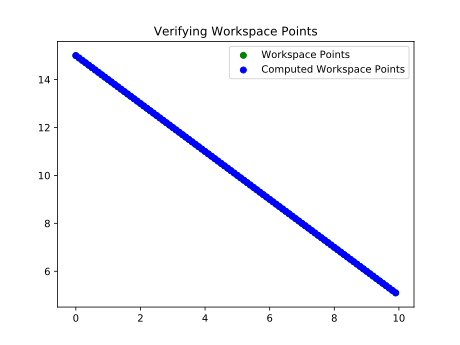
\includepdf[pages={1}]{Problem3_2c.pdf}
  \caption{Problem 3.2}
\end{figure}


\newpage
\section{\textbf{Problem 4.3}}
\lstinputlisting[language=Python]{Problem4_3c.py}

\newpage
\begin{figure}[htbp]
  \centering
  \includepdf[pages={1}]{Problem4_3c.pdf}
  \caption{Problem 4.3}
\end{figure}


\newpage
\section{\textbf{Problem 4.13}}
\lstinputlisting[language=Python]{Problem4_13.py}
Unfortunately Veranda and/or ROS2 (rclpy) has some sort of issue where even when rclpy is shut down correctly topics persist. Nothing is shown in the hidden topic list but they are there. This made simulation near impossible because I had to restart my computer to reset the robot. I had emailed Kali about it but she didn't respond. I eventually sought her out but it was too late. Here is and example of what happens if you kill the program (as demonstrated in the code) and then try to start it back up after a few minutes:

\begin{figure}[htbp]
\centering
\includegraphics[scale=2.0]{VerandaIssue.png}
\caption{Simulation Issues}
\end{figure}


\newpage
\section{\textbf{Problem 4.14}}
\lstinputlisting[language=Python]{Problem4_14.py}

\newpage
\section{\textbf{Text Addition}}
The text addition I have included is \href{https://github.com/macattackftw/ROSwrapper}{ROSwrapper}. The README gives an accurate description of what it is. Example usage is seen \href{https://github.com/macattackftw/ROSwrapper/blob/master/example_basenode.py}{here} and \href{https://github.com/macattackftw/ROSwrapper/blob/master/example_derivednode.py}{here}. ROSwrapper is under development and as such there are some \href{https://github.com/macattackftw/ROSwrapper/issues}{issues}. Please be aware of them while using!


\end{document}
